\newcommand{\templatesdir}{../../../templates}
\newcommand{\template}{template-roteiro-est}
\input{\templatesdir/\template/template}

\newcommand{\content}{Introdução}
\newcommand{\class}{Algoritmos e Estruturas de Dados}
\newcommand{\shortcourse}{45EST}

\begin{document}

\makeheader

Leitura obrigatória:
\begin{itemize}
	\item Capítulo 2 de~\cite{EdelweissAndGalante2009} -- Conceitos básicos.
\end{itemize}
Leitura complementar:
\begin{itemize}
	\item Capítulo 1 de~\cite{Pereira2008} -- Introdução.
\end{itemize}

\medskip

\newtitle{Conceitos básicos}

Algumas definições:
\begin{itemize}
	\item \textbf{Algoritmo:} sequência de passos para realizar uma tarefa.
	\item \textbf{Estrutura de dados:} forma sistemática de organizar e acessar os dados.
\end{itemize}

\textbf{Objetivo:} escolher os melhores componentes para resolver um problema.

\medskip

\textbf{Exemplo}

Jogo para coleta de itens em uma grade (figura abaixo):
\begin{itemize}
	\item \textbf{`X'}: item com valor 100.
	\item \textbf{`O'}: item com valor 200.
	\item Representação do cenário: matriz $n \times n$.
	\item Operações:
	\begin{enumerate}
		\item Varrer ambiente.
		\item Encontrar o item mais próximo.
	\end{enumerate}
\end{itemize}

\begin{figure}[H]
	\centering
	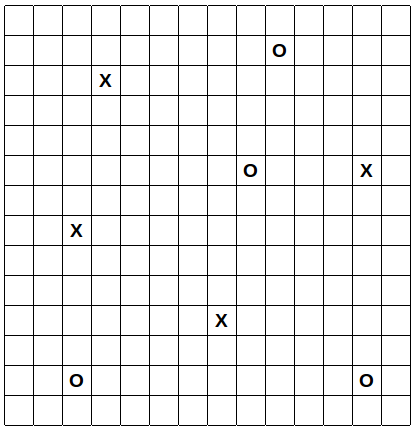
\includegraphics[width=0.6\linewidth]{img/cenario}
\end{figure}

{\color{redtext}
Qual o consumo de memória e tempo de processamento?
\begin{itemize}
	\item Cenário $10 \times 10$.
	\item Cenário $1000 \times 1000$.
	\item Cenário $10000 \times 10000$.
\end{itemize}
}

\block{
	Quanto tempo demora para executar as operações?\\
	Quanta memória é consumida para armazenar o cenário?
}

\textbf{Solução:} usar uma estrutura de dados mais eficiente!

\clearpage

Linguagens de programação fornecem:
\begin{itemize}
	\item Tipos de dados primitivos: inteiro, real, lógico...
	\item Tipos de dados estruturados: arranjos, registros, sequências...
\end{itemize}

\medskip

Usar esses recursos para criar:
\begin{itemize}
	\item TAD (tipo abstrato de dados): estruturas definidas pelo usuário.
	\begin{itemize}
		\item Organização dos dados.
		\item Operações sobre os dados.
	\end{itemize}
\end{itemize}

\medskip

Representação física:
\begin{itemize}
	\item Contiguidade física
	\begin{itemize}
		\item Ex: vetores e matrizes.
		\item Valores armazenados sequencialmente na memória.
		\item $\oplus$ rápido acesso.
		\item $\ominus$ espaço físico estático.
	\end{itemize}
	\item Encadeamento
	\begin{itemize}
		\item Ex: listas, pilhas e filas.
		\item Alocação (não sequencial) dinâmica de memória.
		\item $\oplus$ maleabilidade.
		\item $\ominus$ acesso serial.
	\end{itemize}
\end{itemize}

\clearpage

\newtitle{Atividades}

\begin{enumerate}
	\item Implemente o exemplo do jogo para coleta de itens. Verifique a memória utilizada e o tempo de processamento das operações em função dos diferentes tamanhos da grade. Verifique qual o limite de tamanho capaz de ser processado.
	
	\item Proponha uma nova estrutura de dados, capaz de utilizar menos memória e melhorar o desempenho na execução das operações. Verifique o novo limite de tamanho capaz de ser processado.
\end{enumerate}

\medskip

\newtitle{Referências}
\begingroup
	\footnotesize
	\renewcommand{\chapter}[2]{}%
	\bibliographystyle{apalike}
	\bibliography{../referencias}
\endgroup

\end{document}